\documentclass{article}\usepackage[]{graphicx}\usepackage[]{color}
%% maxwidth is the original width if it is less than linewidth
%% otherwise use linewidth (to make sure the graphics do not exceed the margin)
\makeatletter
\def\maxwidth{ %
  \ifdim\Gin@nat@width>\linewidth
    \linewidth
  \else
    \Gin@nat@width
  \fi
}
\makeatother

\definecolor{fgcolor}{rgb}{0.345, 0.345, 0.345}
\newcommand{\hlnum}[1]{\textcolor[rgb]{0.686,0.059,0.569}{#1}}%
\newcommand{\hlstr}[1]{\textcolor[rgb]{0.192,0.494,0.8}{#1}}%
\newcommand{\hlcom}[1]{\textcolor[rgb]{0.678,0.584,0.686}{\textit{#1}}}%
\newcommand{\hlopt}[1]{\textcolor[rgb]{0,0,0}{#1}}%
\newcommand{\hlstd}[1]{\textcolor[rgb]{0.345,0.345,0.345}{#1}}%
\newcommand{\hlkwa}[1]{\textcolor[rgb]{0.161,0.373,0.58}{\textbf{#1}}}%
\newcommand{\hlkwb}[1]{\textcolor[rgb]{0.69,0.353,0.396}{#1}}%
\newcommand{\hlkwc}[1]{\textcolor[rgb]{0.333,0.667,0.333}{#1}}%
\newcommand{\hlkwd}[1]{\textcolor[rgb]{0.737,0.353,0.396}{\textbf{#1}}}%
\let\hlipl\hlkwb

\usepackage{framed}
\makeatletter
\newenvironment{kframe}{%
 \def\at@end@of@kframe{}%
 \ifinner\ifhmode%
  \def\at@end@of@kframe{\end{minipage}}%
  \begin{minipage}{\columnwidth}%
 \fi\fi%
 \def\FrameCommand##1{\hskip\@totalleftmargin \hskip-\fboxsep
 \colorbox{shadecolor}{##1}\hskip-\fboxsep
     % There is no \\@totalrightmargin, so:
     \hskip-\linewidth \hskip-\@totalleftmargin \hskip\columnwidth}%
 \MakeFramed {\advance\hsize-\width
   \@totalleftmargin\z@ \linewidth\hsize
   \@setminipage}}%
 {\par\unskip\endMakeFramed%
 \at@end@of@kframe}
\makeatother

\definecolor{shadecolor}{rgb}{.97, .97, .97}
\definecolor{messagecolor}{rgb}{0, 0, 0}
\definecolor{warningcolor}{rgb}{1, 0, 1}
\definecolor{errorcolor}{rgb}{1, 0, 0}
\newenvironment{knitrout}{}{} % an empty environment to be redefined in TeX

\usepackage{alltt}
%\usepackage[textwidth=18cm, centering]{geometry}
\usepackage[paper=a4paper,dvips,top=2.5cm,left=2.0cm,right=2.0cm,foot=1cm,bottom=3.2cm]{geometry}
%\usepackage{blindtext}

\setlength{\parindent}{0pt}
\title {ps8}

\author {Kehsin Su Esther 3033114294}
%\textheight=550pt
%\parindent=1pt
\IfFileExists{upquote.sty}{\usepackage{upquote}}{}
\begin{document}
 
\maketitle

\section{Q1}
\subsection{(a)}
As the pdf of exponential distribution has exponential term and pareto is polynomial terms, so when x goes into infinite, exponential distribution will goes to zero faster. Thus, Pareto distribution has heavior tail.
We can use it to do important sample for exponential distribution, which has lighter tail.
As showing is the following graph, y1 has heavior tail.
\begin{knitrout}
\definecolor{shadecolor}{rgb}{0.969, 0.969, 0.969}\color{fgcolor}\begin{kframe}
\begin{alltt}
\hlkwd{require}\hlstd{(sads)}
\end{alltt}


{\ttfamily\noindent\itshape\color{messagecolor}{\#\# Loading required package: sads}}

{\ttfamily\noindent\itshape\color{messagecolor}{\#\# Loading required package: bbmle}}

{\ttfamily\noindent\itshape\color{messagecolor}{\#\# Loading required package: stats4}}\begin{alltt}
\hlkwd{require}\hlstd{(ggplot2)}
\end{alltt}


{\ttfamily\noindent\itshape\color{messagecolor}{\#\# Loading required package: ggplot2}}\begin{alltt}
\hlkwd{require}\hlstd{(reshape2)}
\end{alltt}


{\ttfamily\noindent\itshape\color{messagecolor}{\#\# Loading required package: reshape2}}\begin{alltt}
\hlstd{x} \hlkwb{<-} \hlnum{1}\hlopt{:}\hlnum{100}
\hlstd{pareto} \hlkwb{<-} \hlstd{sads}\hlopt{::}\hlkwd{dpareto}\hlstd{(x,} \hlkwc{shape}\hlstd{=}\hlnum{1}\hlstd{,} \hlkwc{scale} \hlstd{=} \hlkwd{min}\hlstd{(x),} \hlkwc{log} \hlstd{=} \hlnum{FALSE}\hlstd{)}
\hlstd{exponential} \hlkwb{<-} \hlkwd{dexp}\hlstd{(x,} \hlkwc{rate} \hlstd{=} \hlnum{1}\hlstd{,} \hlkwc{log} \hlstd{=} \hlnum{FALSE}\hlstd{)}
\hlstd{df} \hlkwb{<-} \hlkwd{melt}\hlstd{(}\hlkwc{data} \hlstd{=} \hlkwd{data.frame}\hlstd{(x,pareto,exponential),} \hlkwc{id.vars} \hlstd{=} \hlstr{"x"}\hlstd{)}
\hlkwd{colnames}\hlstd{(df)} \hlkwb{<-} \hlkwd{c}\hlstd{(}\hlstr{"x"}\hlstd{,}\hlstr{"Dist"}\hlstd{,}\hlstr{"P_x"}\hlstd{)}
\hlkwd{ggplot}\hlstd{(}\hlkwc{data} \hlstd{= df,} \hlkwd{aes}\hlstd{(}\hlkwc{x} \hlstd{= x,} \hlkwc{y} \hlstd{= P_x,} \hlkwc{colour} \hlstd{= Dist))} \hlopt{+} \hlkwd{geom_line}\hlstd{()}
\end{alltt}
\end{kframe}
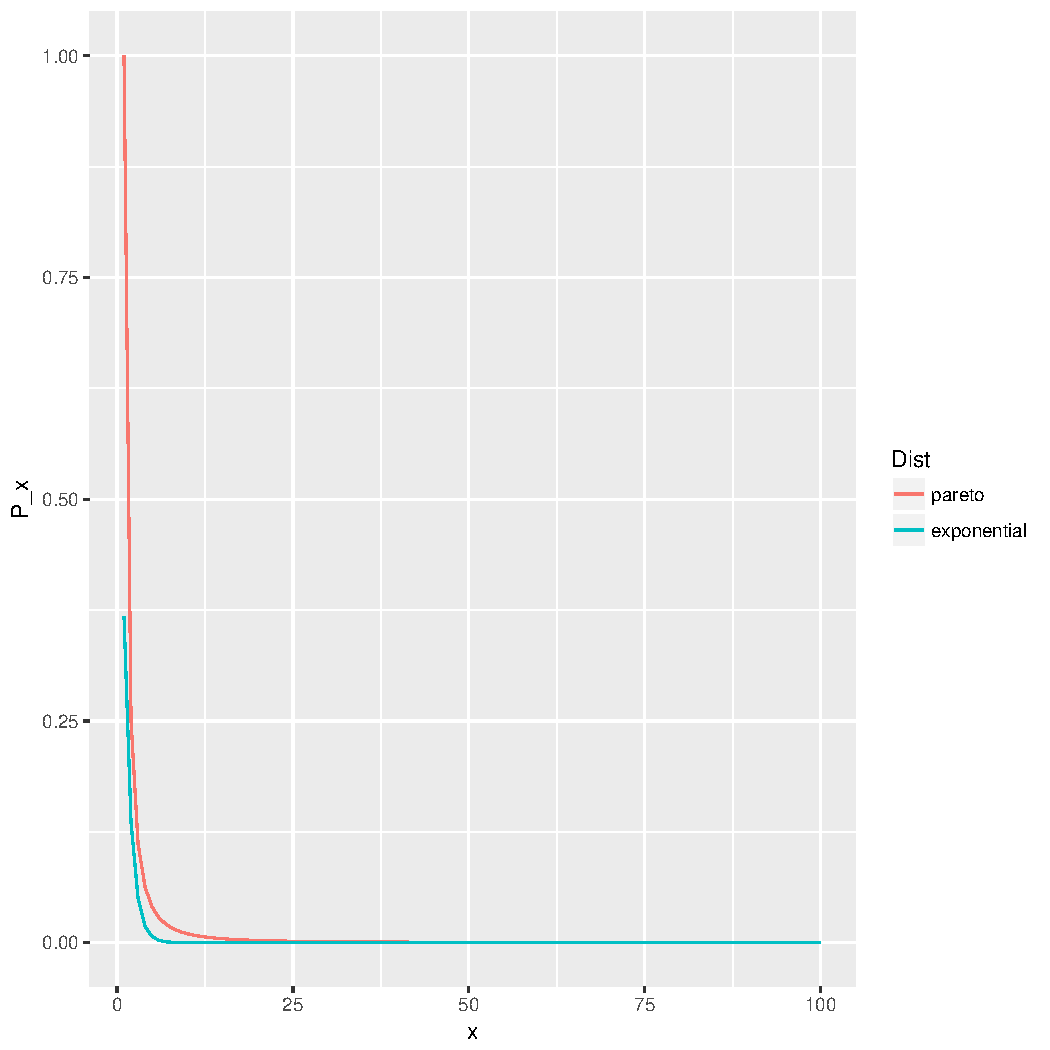
\includegraphics[width=\maxwidth]{figure/unnamed-chunk-1-1} 

\end{knitrout}
\subsection{(b)}
As showing in the following graph, the weight is greater than on the right hand side, but generally, almost all the part has been sampled. Thus, it is fine to use pareto to sampling exponential distribution.i.e. it is fine to use a distribution with heavior tail to sample a distribution with lighter tail, but it won't hold when we switch two distributions to sample.
\begin{knitrout}
\definecolor{shadecolor}{rgb}{0.969, 0.969, 0.969}\color{fgcolor}\begin{kframe}
\begin{alltt}
\hlkwd{library}\hlstd{(tolerance)}
\hlstd{m} \hlkwb{<-} \hlnum{10000}
\hlstd{a} \hlkwb{<-} \hlnum{2}
\hlstd{b} \hlkwb{<-} \hlnum{3}
\hlstd{theta} \hlkwb{<-} \hlnum{1}
\hlstd{shift} \hlkwb{<-} \hlnum{2}
\hlcom{#fx <- r2exp(m, rate = 1, shift = 2)}
\hlstd{x} \hlkwb{<-} \hlkwd{rpareto}\hlstd{(m,} \hlkwc{shape}\hlstd{=a,} \hlkwc{scale} \hlstd{= b)}
\hlstd{hx} \hlkwb{<-} \hlstd{x}
\hlstd{wx} \hlkwb{<-} \hlkwd{d2exp}\hlstd{(x,} \hlkwc{rate} \hlstd{= theta,} \hlkwc{shift} \hlstd{= shift)}\hlopt{/}\hlkwd{dpareto}\hlstd{(x,} \hlkwc{shape}\hlstd{=a,} \hlkwc{scale} \hlstd{= b)} \hlcom{#weight}
\hlkwd{hist}\hlstd{(wx,} \hlkwc{main}\hlstd{=}\hlstr{'Weight distribution'}\hlstd{)}
\end{alltt}
\end{kframe}
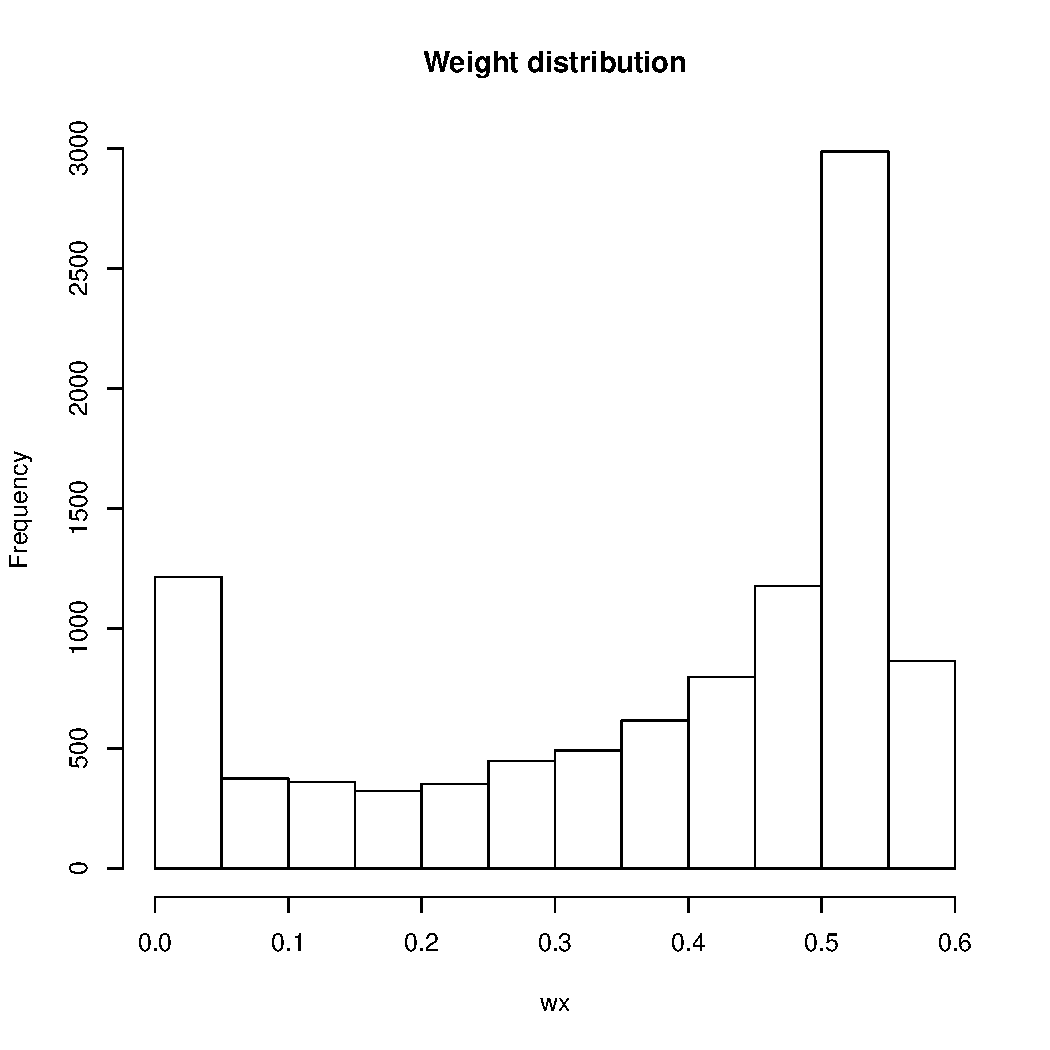
\includegraphics[width=\maxwidth]{figure/unnamed-chunk-2-1} 
\begin{kframe}\begin{alltt}
\hlstd{fx} \hlkwb{<-} \hlstd{hx} \hlopt{*} \hlstd{wx}
\hlkwd{hist}\hlstd{(fx,}\hlkwc{main}\hlstd{=}\hlstr{'Ddistribution of fx'}\hlstd{)}
\hlkwd{lines}\hlstd{(}\hlkwd{density}\hlstd{(fx))}
\end{alltt}
\end{kframe}
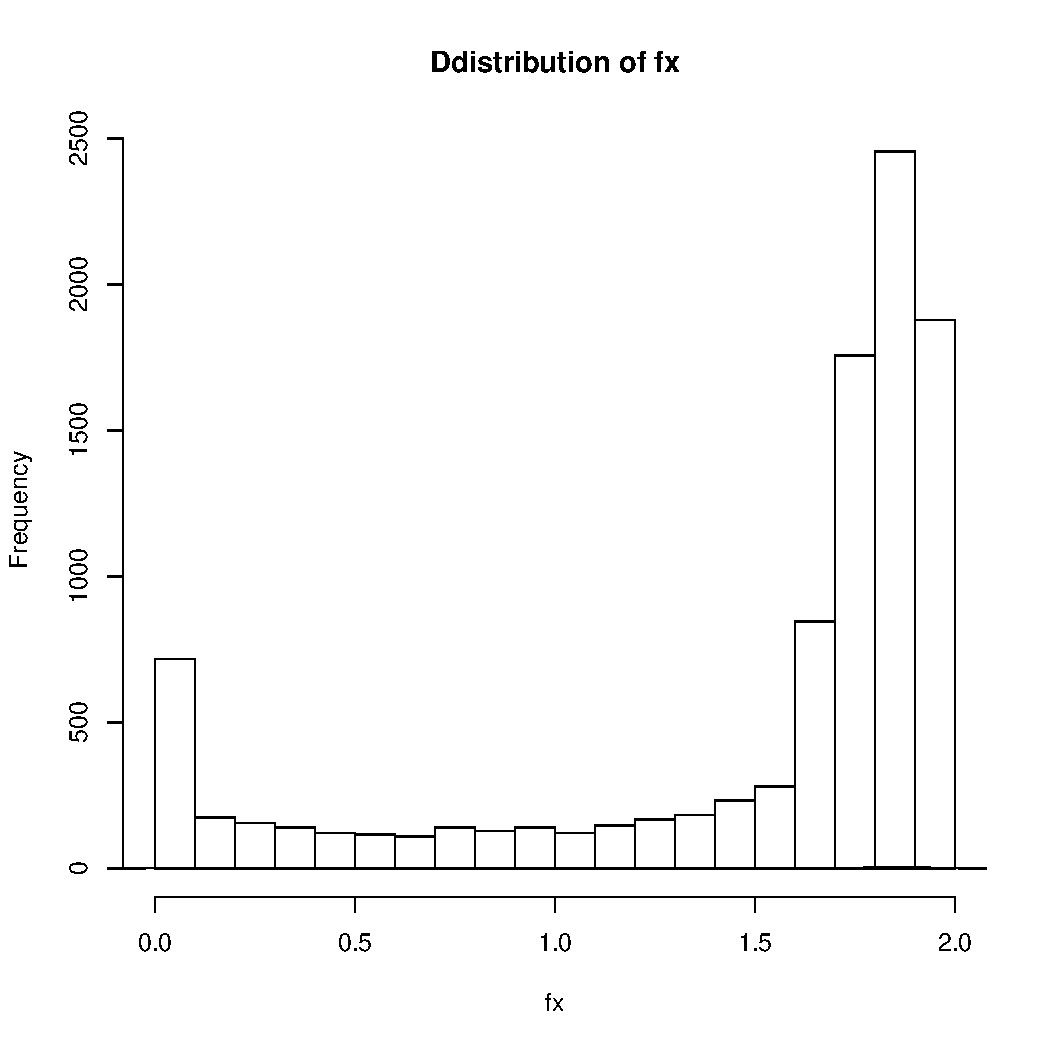
\includegraphics[width=\maxwidth]{figure/unnamed-chunk-2-2} 
\begin{kframe}\begin{alltt}
\hlstd{(ex_hat} \hlkwb{<-} \hlkwd{mean}\hlstd{(fx))}
\end{alltt}
\begin{verbatim}
## [1] 1.482589
\end{verbatim}
\begin{alltt}
\hlstd{(vx_hat} \hlkwb{<-} \hlkwd{var}\hlstd{(fx))}
\end{alltt}
\begin{verbatim}
## [1] 0.3639374
\end{verbatim}
\begin{alltt}
\hlstd{(ex_hat2} \hlkwb{<-} \hlstd{ex_hat}\hlopt{^}\hlnum{2}\hlopt{+}\hlstd{vx_hat)}
\end{alltt}
\begin{verbatim}
## [1] 2.562008
\end{verbatim}
\begin{alltt}
\hlstd{ex} \hlkwb{<-} \hlstd{theta} \hlopt{+} \hlstd{shift}
\hlstd{vx} \hlkwb{<-} \hlstd{theta}
\hlstd{mse} \hlkwb{<-} \hlstd{(ex_hat}\hlopt{-}\hlstd{ex)}\hlopt{^}\hlnum{2}
\end{alltt}
\end{kframe}
\end{knitrout}

\subsection{(c)}
As showing in the following graph, as the one with heavior divide the one with ligter tail will make the value go to infinite, so as the histgram, it center mostly on the left sight which close to zero.
\begin{knitrout}
\definecolor{shadecolor}{rgb}{0.969, 0.969, 0.969}\color{fgcolor}\begin{kframe}
\begin{alltt}
\hlkwd{library}\hlstd{(tolerance)}
\hlstd{m} \hlkwb{<-} \hlnum{10000}
\hlstd{x} \hlkwb{<-} \hlkwd{r2exp}\hlstd{(m,} \hlkwc{rate} \hlstd{= theta,} \hlkwc{shift} \hlstd{= shift)}
\hlcom{#x <- rpareto(m, shape= a, scale = b)}
\hlstd{hx} \hlkwb{<-} \hlstd{x}
\hlstd{wx} \hlkwb{<-} \hlkwd{dpareto}\hlstd{(x,} \hlkwc{shape}\hlstd{=a,} \hlkwc{scale} \hlstd{= b)}\hlopt{/}\hlkwd{d2exp}\hlstd{(x,} \hlkwc{rate} \hlstd{= theta,} \hlkwc{shift} \hlstd{= shift)} \hlcom{#weight}
\hlkwd{hist}\hlstd{(wx,} \hlkwc{main}\hlstd{=}\hlstr{'Weight distribution'}\hlstd{)}
\end{alltt}
\end{kframe}
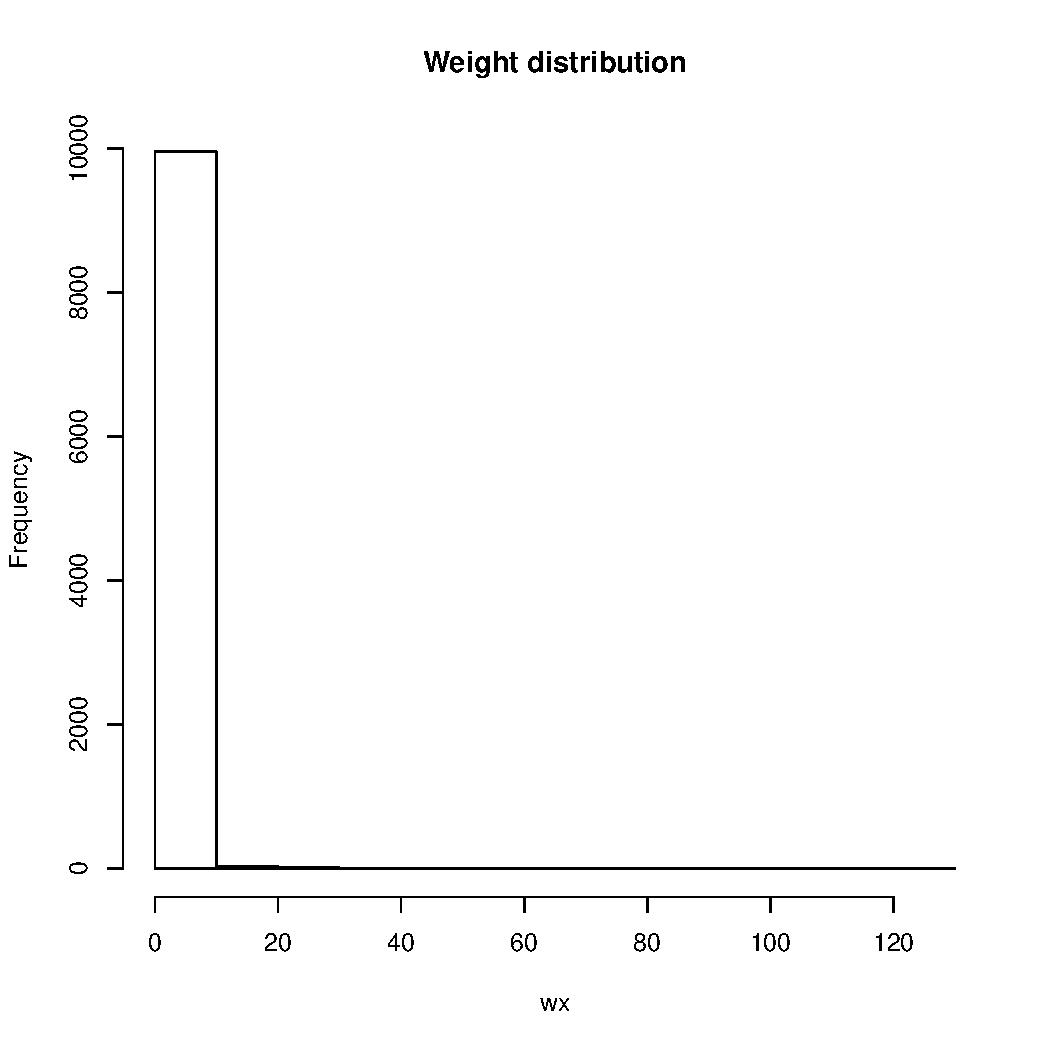
\includegraphics[width=\maxwidth]{figure/unnamed-chunk-3-1} 
\begin{kframe}\begin{alltt}
\hlstd{fx} \hlkwb{<-} \hlstd{hx} \hlopt{*} \hlstd{wx}
\hlkwd{hist}\hlstd{(fx,}\hlkwc{main}\hlstd{=}\hlstr{'Distribution of fx'}\hlstd{)}
\hlkwd{lines}\hlstd{(}\hlkwd{density}\hlstd{(fx))}
\end{alltt}
\end{kframe}
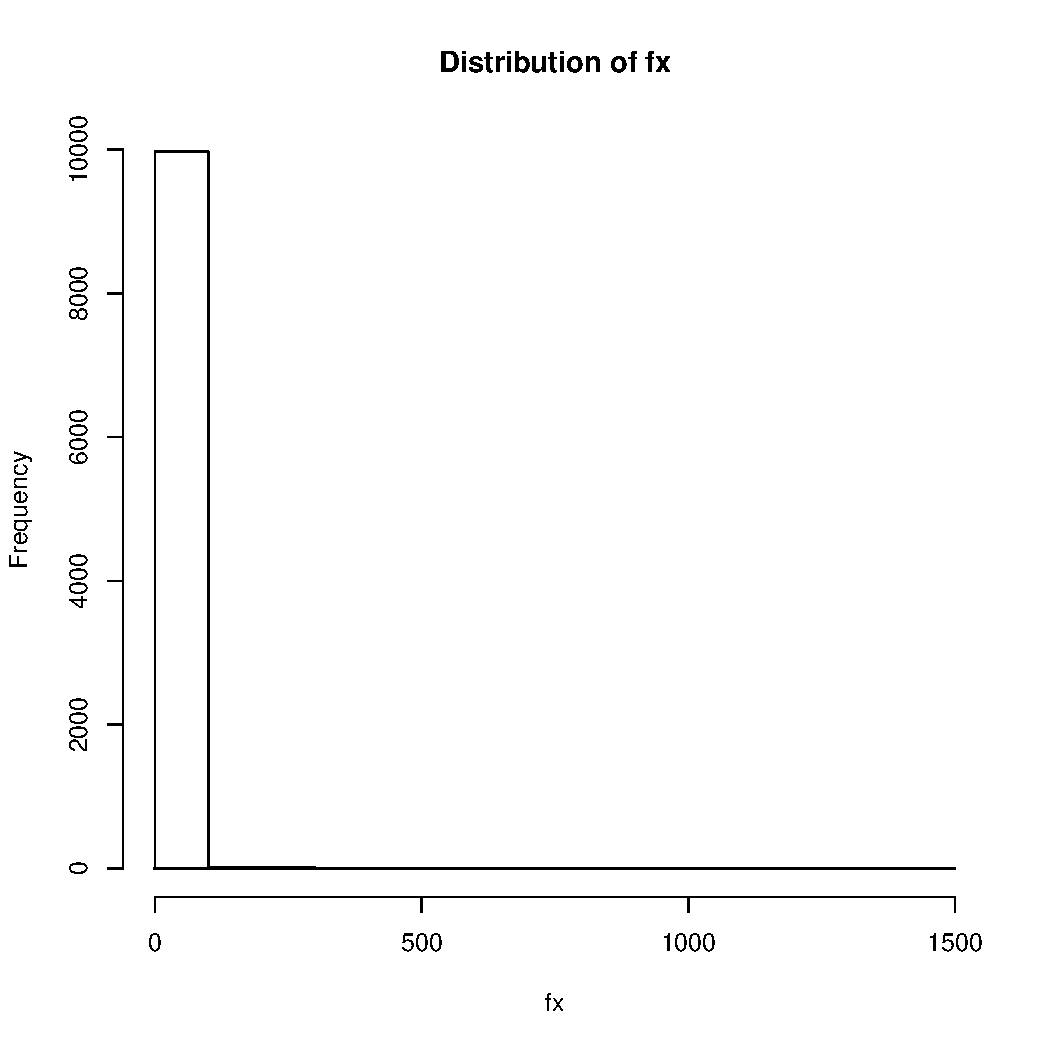
\includegraphics[width=\maxwidth]{figure/unnamed-chunk-3-2} 
\begin{kframe}\begin{alltt}
\hlstd{(ex_hat} \hlkwb{<-} \hlkwd{mean}\hlstd{(fx))}
\end{alltt}
\begin{verbatim}
## [1] 4.29801
\end{verbatim}
\begin{alltt}
\hlstd{(vx_hat} \hlkwb{<-} \hlkwd{var}\hlstd{(fx))}
\end{alltt}
\begin{verbatim}
## [1] 402.0106
\end{verbatim}
\begin{alltt}
\hlstd{(ex_hat2} \hlkwb{<-} \hlstd{ex_hat}\hlopt{^}\hlnum{2}\hlopt{+}\hlstd{vx_hat)}
\end{alltt}
\begin{verbatim}
## [1] 420.4835
\end{verbatim}
\begin{alltt}
\hlstd{(ex} \hlkwb{<-} \hlstd{b}\hlopt{*}\hlstd{a}\hlopt{/}\hlstd{(b}\hlopt{-}\hlnum{1}\hlstd{))}
\end{alltt}
\begin{verbatim}
## [1] 3
\end{verbatim}
\begin{alltt}
\hlstd{(vx} \hlkwb{<-} \hlstd{b}\hlopt{*}\hlstd{a}\hlopt{^}\hlnum{2}\hlopt{/}\hlstd{(b}\hlopt{-}\hlnum{1}\hlstd{)}\hlopt{^}\hlnum{2}\hlopt{/}\hlstd{(b}\hlopt{-}\hlnum{2}\hlstd{))}
\end{alltt}
\begin{verbatim}
## [1] 3
\end{verbatim}
\begin{alltt}
\hlstd{ex2} \hlkwb{<-} \hlstd{ex}\hlopt{^}\hlnum{2}\hlopt{+}\hlstd{vx}
\hlstd{(mse} \hlkwb{<-} \hlstd{(ex_hat}\hlopt{-}\hlstd{ex)}\hlopt{^}\hlnum{2}\hlstd{)}
\end{alltt}
\begin{verbatim}
## [1] 1.68483
\end{verbatim}
\end{kframe}
\end{knitrout}
\section{Q2}
First, fix a dimension and plot some 3d plot to observe how does the curve looks like. Then, we found that it's hard to identify the lowest point. Contour make it easier to identify to lowest point. With differnet slice, we plot different picture and choose to possible point to that dimension.
\begin{knitrout}
\definecolor{shadecolor}{rgb}{0.969, 0.969, 0.969}\color{fgcolor}\begin{kframe}
\begin{alltt}
\hlkwd{library}\hlstd{(rgl)}
\hlkwd{library}\hlstd{(graphics)}
\hlkwd{library}\hlstd{(ggplot2)}
\hlcom{## problem 2}
\hlstd{theta} \hlkwb{<-} \hlkwa{function}\hlstd{(}\hlkwc{x1}\hlstd{,}\hlkwc{x2}\hlstd{)} \hlkwd{atan2}\hlstd{(x2, x1)}\hlopt{/}\hlstd{(}\hlnum{2}\hlopt{*}\hlstd{pi)}

\hlstd{f} \hlkwb{<-} \hlkwa{function}\hlstd{(}\hlkwc{x}\hlstd{) \{}
  \hlstd{f1} \hlkwb{<-} \hlnum{10}\hlopt{*}\hlstd{(x[[}\hlnum{3}\hlstd{]]} \hlopt{-} \hlnum{10}\hlopt{*}\hlkwd{theta}\hlstd{(x[[}\hlnum{1}\hlstd{]],x[[}\hlnum{2}\hlstd{]]))}
  \hlstd{f2} \hlkwb{<-} \hlnum{10}\hlopt{*}\hlstd{(}\hlkwd{sqrt}\hlstd{(x[[}\hlnum{1}\hlstd{]]}\hlopt{^}\hlnum{2} \hlopt{+} \hlstd{x[[}\hlnum{2}\hlstd{]]}\hlopt{^}\hlnum{2}\hlstd{)} \hlopt{-} \hlnum{1}\hlstd{)}
  \hlstd{f3} \hlkwb{<-} \hlstd{x[[}\hlnum{3}\hlstd{]]}
  \hlkwd{return}\hlstd{(f1}\hlopt{^}\hlnum{2} \hlopt{+} \hlstd{f2}\hlopt{^}\hlnum{2} \hlopt{+} \hlstd{f3}\hlopt{^}\hlnum{2}\hlstd{)}
\hlstd{\}}
\hlcom{## calculate the minimum}

\hlstd{f2} \hlkwb{<-} \hlkwa{function}\hlstd{(}\hlkwc{x}\hlstd{) \{}
  \hlstd{f1} \hlkwb{<-} \hlnum{10}\hlopt{*}\hlstd{(x[}\hlnum{3}\hlstd{]} \hlopt{-} \hlnum{10}\hlopt{*}\hlkwd{theta}\hlstd{(x[}\hlnum{1}\hlstd{],x[}\hlnum{2}\hlstd{]))}
  \hlstd{f2} \hlkwb{<-} \hlnum{10}\hlopt{*}\hlstd{(}\hlkwd{sqrt}\hlstd{(x[}\hlnum{1}\hlstd{]}\hlopt{^}\hlnum{2} \hlopt{+} \hlstd{x[}\hlnum{2}\hlstd{]}\hlopt{^}\hlnum{2}\hlstd{)} \hlopt{-} \hlnum{1}\hlstd{)}
  \hlstd{f3} \hlkwb{<-} \hlstd{x[}\hlnum{3}\hlstd{]}
  \hlkwd{return}\hlstd{(f1}\hlopt{^}\hlnum{2} \hlopt{+} \hlstd{f2}\hlopt{^}\hlnum{2} \hlopt{+} \hlstd{f3}\hlopt{^}\hlnum{2}\hlstd{)}
\hlstd{\}}
\hlstd{my_filled_plot} \hlkwb{<-} \hlkwa{function}\hlstd{(}\hlkwc{x}\hlstd{) \{}
  \hlstd{range1} \hlkwb{<-} \hlkwd{seq}\hlstd{(}\hlopt{-}\hlnum{3}\hlopt{*}\hlstd{pi,}\hlnum{3}\hlopt{*}\hlstd{pi,}\hlnum{1}\hlstd{)}
  \hlstd{n1} \hlkwb{<-} \hlkwd{length}\hlstd{(range1)}
  \hlstd{h} \hlkwb{<-} \hlkwd{matrix}\hlstd{(}\hlnum{NA}\hlstd{,n1,n1)}
  \hlstd{d3} \hlkwb{<-} \hlstd{x}
  \hlkwa{for} \hlstd{(i} \hlkwa{in} \hlstd{range1)\{}
    \hlkwa{for}\hlstd{(j} \hlkwa{in} \hlstd{range1)\{}
      \hlstd{h[i,j]} \hlkwb{<-} \hlkwd{f2}\hlstd{(}\hlkwd{c}\hlstd{(i,j,d3))}
    \hlstd{\}}

  \hlstd{\}}
  \hlkwd{filled.contour}\hlstd{(range1,range1,h,} \hlkwc{color} \hlstd{= terrain.colors)}

\hlstd{\}}

\hlstd{range1} \hlkwb{<-} \hlkwd{seq}\hlstd{(}\hlopt{-}\hlnum{3}\hlopt{*}\hlstd{pi,}\hlnum{3}\hlopt{*}\hlstd{pi,}\hlnum{1}\hlstd{)}
\hlstd{n1} \hlkwb{<-} \hlkwd{length}\hlstd{(range1)}
\hlstd{h} \hlkwb{<-} \hlkwd{matrix}\hlstd{(}\hlnum{NA}\hlstd{,n1,n1)}
\hlstd{d3} \hlkwb{<-} \hlstd{pi}
\hlkwa{for} \hlstd{(i} \hlkwa{in} \hlstd{range1)\{}
  \hlkwa{for}\hlstd{(j} \hlkwa{in} \hlstd{range1)\{}
    \hlstd{h[i,j]} \hlkwb{<-} \hlkwd{f2}\hlstd{(}\hlkwd{c}\hlstd{(i,j,d3))}
  \hlstd{\}}
\hlstd{\}}
\hlkwd{require}\hlstd{(lattice)}
\end{alltt}


{\ttfamily\noindent\itshape\color{messagecolor}{\#\# Loading required package: lattice}}\begin{alltt}
\hlcom{#wireframe(h, drape=T, col.regions=rainbow(10000000))}
\hlkwd{wireframe}\hlstd{(h,} \hlkwc{drape}\hlstd{=T)}
\end{alltt}
\end{kframe}
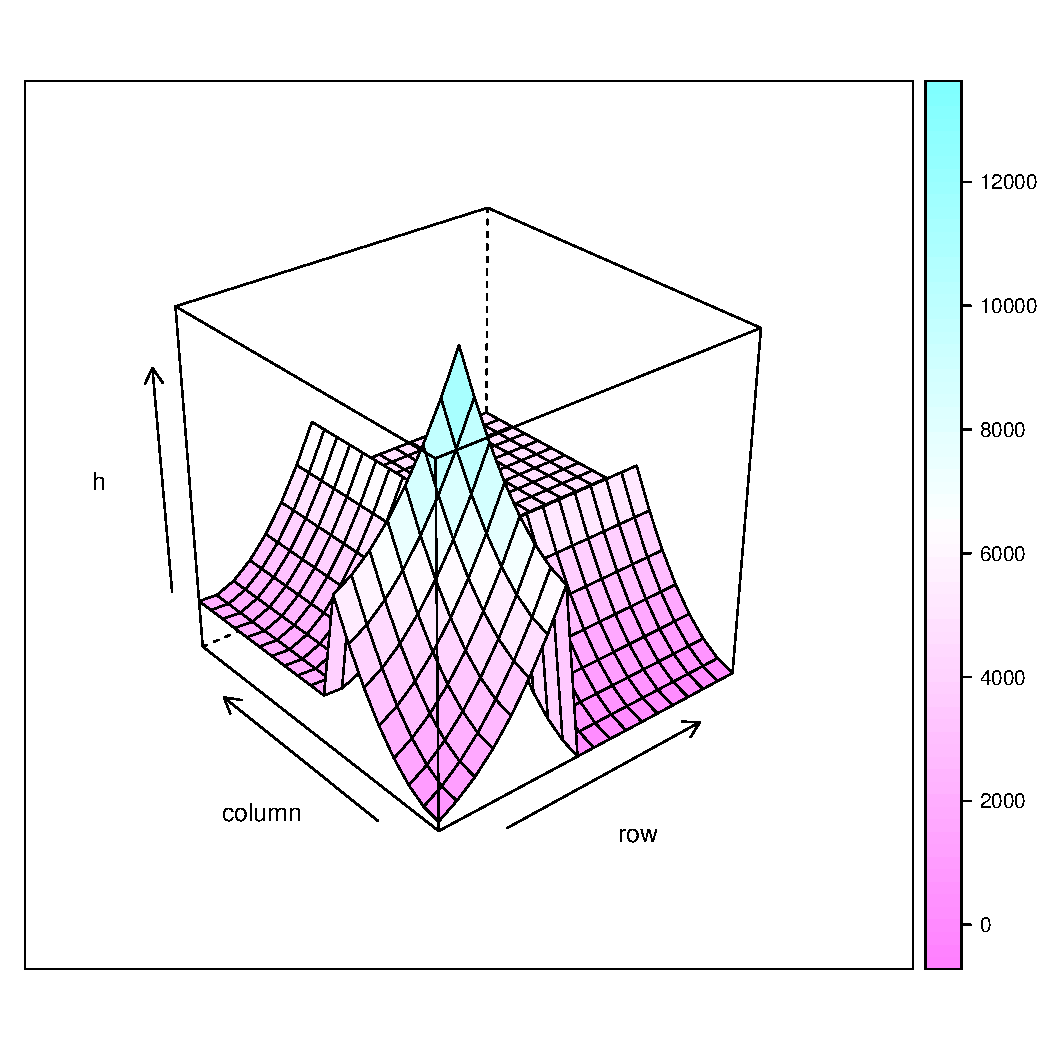
\includegraphics[width=\maxwidth]{figure/unnamed-chunk-4-1} 
\begin{kframe}\begin{alltt}
\hlkwd{persp}\hlstd{(range1,range1,h,}\hlkwc{xlim} \hlstd{=} \hlkwd{range}\hlstd{(}\hlopt{-}\hlnum{3}\hlopt{*}\hlstd{pi,}\hlnum{3}\hlopt{*}\hlstd{pi),} \hlkwc{ylim} \hlstd{=} \hlkwd{range}\hlstd{(}\hlopt{-}\hlnum{3}\hlopt{*}\hlstd{pi,}\hlnum{3}\hlopt{*}\hlstd{pi))}
\end{alltt}
\end{kframe}
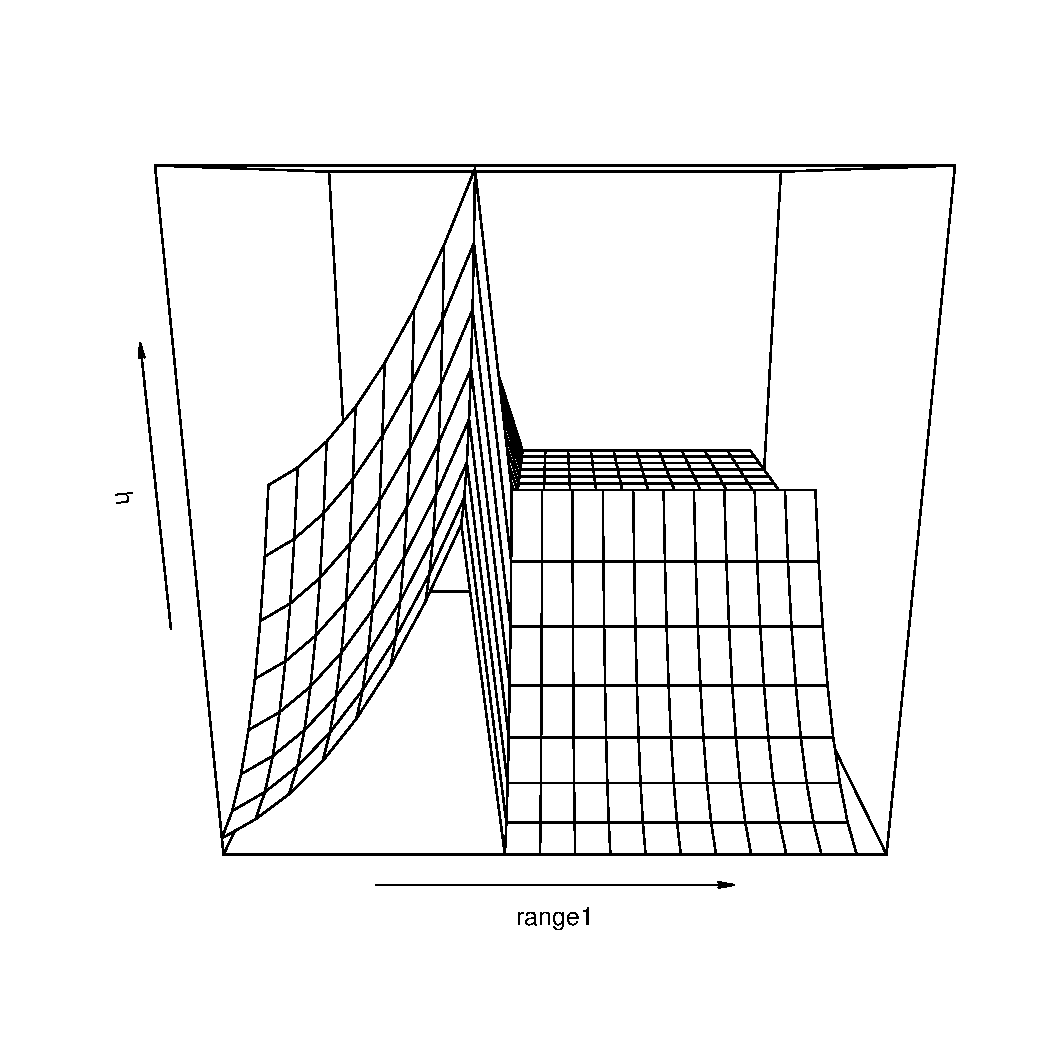
\includegraphics[width=\maxwidth]{figure/unnamed-chunk-4-2} 
\begin{kframe}\begin{alltt}
\hlkwd{contour}\hlstd{(range1,range1,h)}
\end{alltt}
\end{kframe}
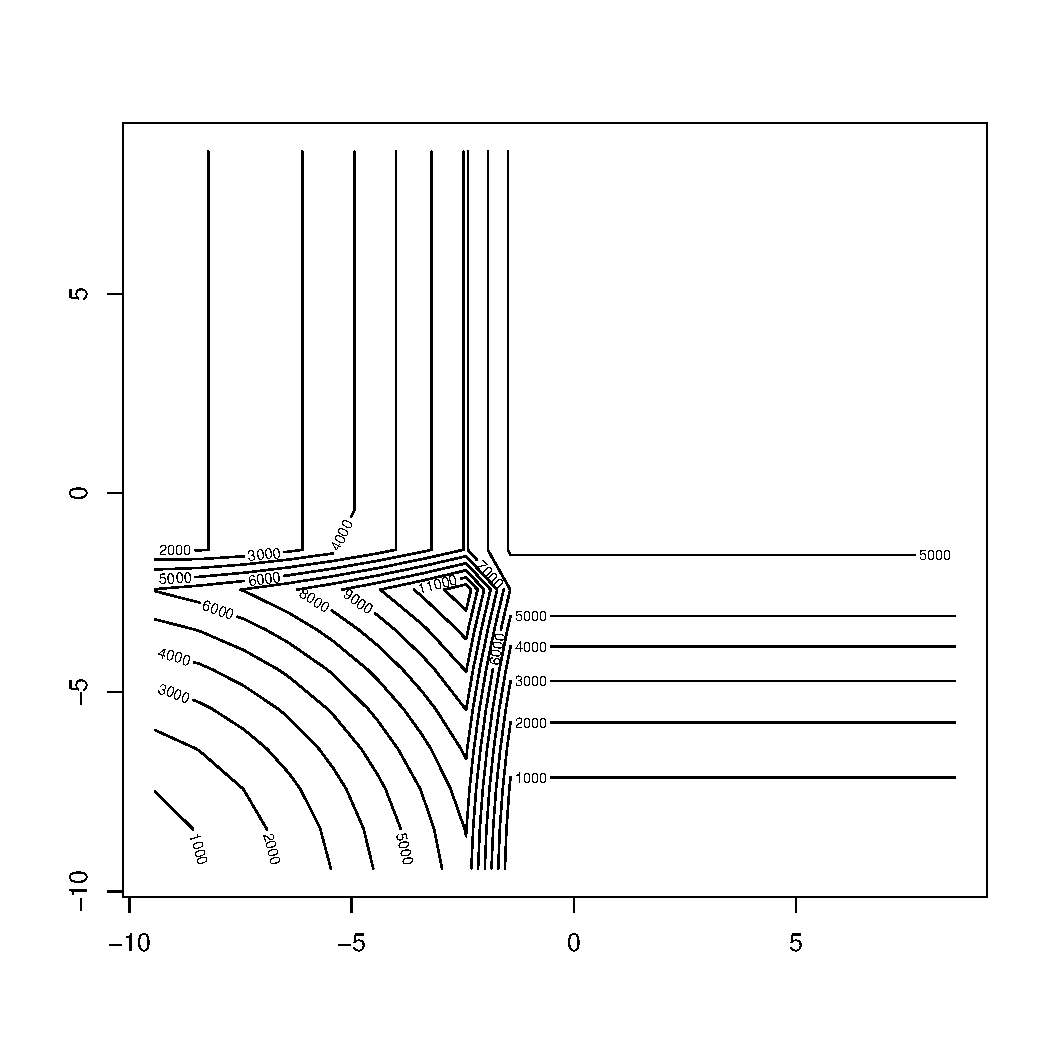
\includegraphics[width=\maxwidth]{figure/unnamed-chunk-4-3} 
\begin{kframe}\begin{alltt}
\hlkwd{my_filled_plot}\hlstd{(pi)}
\end{alltt}
\end{kframe}
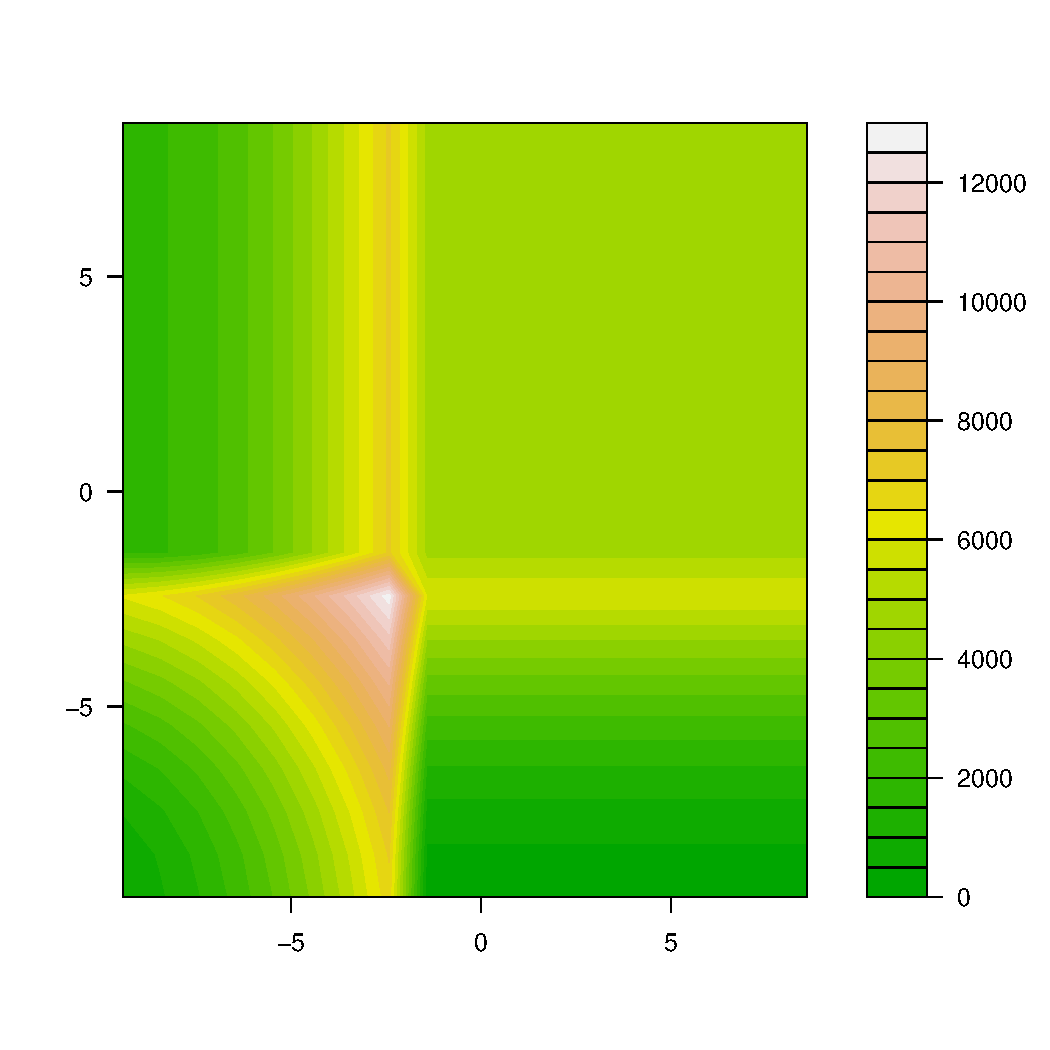
\includegraphics[width=\maxwidth]{figure/unnamed-chunk-4-4} 
\begin{kframe}\begin{alltt}
\hlcom{# require(rgl)}
\hlcom{# open3d()}
\hlcom{# rgl.surface(range1,range1,h)}

\hlkwd{require}\hlstd{(plot3D)}
\end{alltt}


{\ttfamily\noindent\itshape\color{messagecolor}{\#\# Loading required package: plot3D}}\begin{alltt}
\hlcom{#persp3D(z = h, theta = 120)}

\hlkwd{library}\hlstd{(graphics)}
\hlkwd{library}\hlstd{(ggplot2)}
\hlstd{myplot1} \hlkwb{<-} \hlkwa{function}\hlstd{(}\hlkwc{x1}\hlstd{,}\hlkwc{x2}\hlstd{,}\hlkwc{x3}\hlstd{)\{}
  \hlstd{x} \hlkwb{<-} \hlkwd{list}\hlstd{(x1 ,x2, x3)}
  \hlstd{z} \hlkwb{<-} \hlkwd{f}\hlstd{(x)}
  \hlstd{df} \hlkwb{<-} \hlkwd{data.frame}\hlstd{(x1,x2,z)}
  \hlkwd{plot3d}\hlstd{(df)}
  \hlstd{\}}

\hlstd{myplot} \hlkwb{<-} \hlkwa{function}\hlstd{(}\hlkwc{x1}\hlstd{,}\hlkwc{x2}\hlstd{,}\hlkwc{x3}\hlstd{)\{}
  \hlstd{x} \hlkwb{<-} \hlkwd{list}\hlstd{(x1 ,x2, x3)}
  \hlstd{z} \hlkwb{<-} \hlkwd{f}\hlstd{(x)}
  \hlstd{height} \hlkwb{<-}\hlkwd{cut}\hlstd{(z,}\hlnum{20}\hlstd{)}
  \hlstd{df} \hlkwb{<-} \hlkwd{data.frame}\hlstd{(x1,x2,z)}
  \hlstd{(}\hlkwd{ggplot}\hlstd{(}\hlkwc{data}\hlstd{=df,} \hlkwd{aes}\hlstd{(}\hlkwc{x}\hlstd{=x1,} \hlkwc{y}\hlstd{=x2,} \hlkwc{z}\hlstd{=z))}
  \hlopt{+} \hlkwd{geom_point}\hlstd{(}\hlkwd{aes}\hlstd{(}\hlkwc{colour}\hlstd{=height))}
  \hlopt{+} \hlkwd{geom_density2d}\hlstd{()}

  \hlstd{)}
\hlstd{\}}
\hlcom{#test fixed x3 in four different value: 0,pi/2, 3pi/2, 2pi}
\hlcom{#since we need to calculate tan of x1,x2, so it's better to set x3 within the range from -2pi to 2pi to maintan the same scale}
\hlstd{x1} \hlkwb{<-} \hlkwd{seq}\hlstd{(}\hlopt{-}\hlnum{2}\hlopt{*}\hlstd{pi,} \hlnum{2}\hlopt{*}\hlstd{pi,} \hlkwc{length}\hlstd{=} \hlnum{100}\hlstd{)}
\hlstd{x2} \hlkwb{<-} \hlkwd{seq}\hlstd{(}\hlopt{-}\hlnum{2}\hlopt{*}\hlstd{pi,} \hlnum{2}\hlopt{*}\hlstd{pi,} \hlkwc{length}\hlstd{=} \hlnum{100}\hlstd{)}
\hlstd{x3} \hlkwb{<-} \hlkwd{rep}\hlstd{(}\hlnum{0}\hlstd{,}\hlnum{100}\hlstd{)}
\hlcom{#myplot(x1,x2,x3)}

\hlstd{x3} \hlkwb{<-} \hlkwd{rep}\hlstd{(pi,}\hlnum{100}\hlstd{)}
\hlcom{#myplot(x1,x2,x3)}

\hlstd{x3} \hlkwb{<-} \hlkwd{rep}\hlstd{(}\hlnum{2}\hlopt{*}\hlstd{pi,}\hlnum{100}\hlstd{)}
\hlcom{#myplot(x1,x2,x3)}

\hlstd{x3} \hlkwb{<-} \hlkwd{rep}\hlstd{(}\hlopt{-}\hlstd{pi,}\hlnum{100}\hlstd{)}
\hlcom{#myplot(x1,x2,x3)}

\hlstd{x3} \hlkwb{<-} \hlkwd{rep}\hlstd{(}\hlopt{-}\hlnum{2}\hlopt{*}\hlstd{pi,}\hlnum{100}\hlstd{)}
\hlcom{#myplot(x1,x2,x3)}

\hlcom{# par(mfrow=c(2,2))}



\hlcom{#When fixed x3 equal to zero, the color chenge at about point (0,0) and point (2.5,2.5), so we set these two point to test }
\hlstd{p1} \hlkwb{<-} \hlkwd{c}\hlstd{(}\hlnum{0}\hlstd{,}\hlnum{0}\hlstd{,}\hlnum{0}\hlstd{)}
\hlkwd{optim}\hlstd{(p1,f)}\hlopt{$}\hlstd{value}
\end{alltt}
\begin{verbatim}
## [1] 1.876851e-05
\end{verbatim}
\begin{alltt}
\hlkwd{nlm}\hlstd{(f,p1)}\hlopt{$}\hlstd{minimum}
\end{alltt}
\begin{verbatim}
## [1] 100
\end{verbatim}
\begin{alltt}
\hlstd{p2} \hlkwb{<-} \hlkwd{c}\hlstd{(}\hlnum{2.5}\hlstd{,}\hlnum{2.5}\hlstd{,}\hlnum{0}\hlstd{)}
\hlkwd{optim}\hlstd{(p2,f)}\hlopt{$}\hlstd{value}
\end{alltt}
\begin{verbatim}
## [1] 3.217961e-06
\end{verbatim}
\begin{alltt}
\hlkwd{nlm}\hlstd{(f,p2)}\hlopt{$}\hlstd{minimum} \hlcom{#better}
\end{alltt}
\begin{verbatim}
## [1] 3.348995e-19
\end{verbatim}
\begin{alltt}
\hlcom{#When fixed x3 equal to pi, the color chenge at about point (0,0) and point (2,2), so we set these two point to test }
\hlstd{p3} \hlkwb{<-} \hlkwd{c}\hlstd{(}\hlnum{0}\hlstd{,}\hlnum{0}\hlstd{,pi)}
\hlkwd{optim}\hlstd{(p3,f)}\hlopt{$}\hlstd{value}
\end{alltt}
\begin{verbatim}
## [1] 1.199054e-05
\end{verbatim}
\begin{alltt}
\hlkwd{nlm}\hlstd{(f,p3)}\hlopt{$}\hlstd{minimum}
\end{alltt}
\begin{verbatim}
## [1] 149.8989
\end{verbatim}
\begin{alltt}
\hlstd{p4} \hlkwb{<-} \hlkwd{c}\hlstd{(}\hlnum{2}\hlstd{,}\hlnum{2}\hlstd{,pi)}
\hlkwd{optim}\hlstd{(p4,f)}\hlopt{$}\hlstd{value}
\end{alltt}
\begin{verbatim}
## [1] 9.900303e-07
\end{verbatim}
\begin{alltt}
\hlkwd{nlm}\hlstd{(f,p4)}\hlopt{$}\hlstd{minimum} \hlcom{#better}
\end{alltt}
\begin{verbatim}
## [1] 1.294807e-18
\end{verbatim}
\begin{alltt}
\hlcom{#When fixed x3 equal to pi*2, the color chenge at about point (0,0) and point (2,2), so we set these two point to test }
\hlstd{p5} \hlkwb{<-} \hlkwd{c}\hlstd{(}\hlnum{0}\hlstd{,}\hlnum{0}\hlstd{,}\hlnum{2}\hlopt{*}\hlstd{pi)}
\hlkwd{optim}\hlstd{(p5,f)}\hlopt{$}\hlstd{value}
\end{alltt}
\begin{verbatim}
## [1] 1.253867e-05
\end{verbatim}
\begin{alltt}
\hlkwd{nlm}\hlstd{(f,p5)}\hlopt{$}\hlstd{minimum}
\end{alltt}
\begin{verbatim}
## [1] 1569.631
\end{verbatim}
\begin{alltt}
\hlstd{p6} \hlkwb{<-} \hlkwd{c}\hlstd{(}\hlnum{2}\hlstd{,}\hlnum{2}\hlstd{,}\hlnum{2}\hlopt{*}\hlstd{pi)}
\hlkwd{optim}\hlstd{(p6,f)}\hlopt{$}\hlstd{value}
\end{alltt}
\begin{verbatim}
## [1] 1.264891e-05
\end{verbatim}
\begin{alltt}
\hlkwd{nlm}\hlstd{(f,p6)}\hlopt{$}\hlstd{minimum} \hlcom{#better}
\end{alltt}
\begin{verbatim}
## [1] 2.129973e-18
\end{verbatim}
\begin{alltt}
\hlcom{#When fixed x3 equal to -pi, the color chenge at about point (0,0) and point (-2,6), so we set these two point to test }
\hlstd{p7} \hlkwb{<-} \hlkwd{c}\hlstd{(}\hlopt{-}\hlnum{2}\hlstd{,}\hlopt{-}\hlnum{2}\hlstd{,}\hlopt{-}\hlstd{pi)}
\hlkwd{optim}\hlstd{(p7,f)}\hlopt{$}\hlstd{value}
\end{alltt}
\begin{verbatim}
## [1] 4.910886e-06
\end{verbatim}
\begin{alltt}
\hlkwd{nlm}\hlstd{(f,p7)}\hlopt{$}\hlstd{minimum} \hlcom{#better}
\end{alltt}
\begin{verbatim}
## [1] 1.700644e-08
\end{verbatim}
\begin{alltt}
\hlstd{p8} \hlkwb{<-} \hlkwd{c}\hlstd{(}\hlnum{0}\hlstd{,}\hlnum{0}\hlstd{,}\hlopt{-}\hlstd{pi)}
\hlkwd{optim}\hlstd{(p8,f)}\hlopt{$}\hlstd{value}
\end{alltt}
\begin{verbatim}
## [1] 6.625893e-06
\end{verbatim}
\begin{alltt}
\hlkwd{nlm}\hlstd{(f,p8)}\hlopt{$}\hlstd{minimum}
\end{alltt}
\begin{verbatim}
## [1] 150.5356
\end{verbatim}
\begin{alltt}
\hlcom{#When fixed x3 equal to -2*pi, the color chenge at about point (0,0) and point (-1.5,-1.5), so we set these two point to test }
\hlstd{p9} \hlkwb{<-} \hlkwd{c}\hlstd{(}\hlopt{-}\hlnum{1.5}\hlstd{,}\hlopt{-}\hlnum{1.5}\hlstd{,}\hlopt{-}\hlstd{pi}\hlopt{*}\hlnum{2}\hlstd{)}
\hlkwd{optim}\hlstd{(p9,f)}\hlopt{$}\hlstd{value}
\end{alltt}
\begin{verbatim}
## [1] 5.694121e-05
\end{verbatim}
\begin{alltt}
\hlkwd{nlm}\hlstd{(f,p9)}\hlopt{$}\hlstd{minimum} \hlcom{#better}
\end{alltt}
\begin{verbatim}
## [1] 1.700871e-08
\end{verbatim}
\begin{alltt}
\hlstd{p10} \hlkwb{<-} \hlkwd{c}\hlstd{(}\hlnum{0}\hlstd{,}\hlnum{0}\hlstd{,}\hlopt{-}\hlstd{pi}\hlopt{*}\hlnum{2}\hlstd{)}
\hlkwd{optim}\hlstd{(p10,f)}\hlopt{$}\hlstd{value}
\end{alltt}
\begin{verbatim}
## [1] 1.179725e-05
\end{verbatim}
\begin{alltt}
\hlkwd{nlm}\hlstd{(f,p10)}\hlopt{$}\hlstd{minimum}
\end{alltt}
\begin{verbatim}
## [1] 1569.67
\end{verbatim}
\begin{alltt}
\hlcom{#As showing above, set p6 as beginning point will generates the mimimum value, so we choose it with nlm to calcuate the mimimum value}
\hlkwd{nlm}\hlstd{(f,p2)}
\end{alltt}
\begin{verbatim}
## $minimum
## [1] 3.348995e-19
## 
## $estimate
## [1] 1.000000e+00 1.820975e-10 2.380022e-10
## 
## $gradient
## [1] -1.977529e-09  1.649318e-08 -9.886966e-09
## 
## $code
## [1] 1
## 
## $iterations
## [1] 22
\end{verbatim}
\end{kframe}
\end{knitrout}

\section{Q3}
\subsection{(a)}
Details append at last page. The first step is to condidition on the coefficients and calcuate the expectation of log likelihood funciton. Second, we can take log and solve the equation to get the recursive solution of coefficients. The key concept is that the coefficent can be evalued similar like general regression coefficent, but the cencor part is estimated by specific expectation value to start em algorithm, and variance also has a special term for the cencor part.
\subsection{(b)}
The start point can be set by uncencoring data. We can use summary of "lm" function to get beta0, beta1 and sigma as an initial point. Then use such coefficeints to estimate the cencor data and keep updating the coefficients until to the coefficients very close to the coefficients we obtain in the previous step. Then we can get the final solution.
\subsection{(c)}
\begin{knitrout}
\definecolor{shadecolor}{rgb}{0.969, 0.969, 0.969}\color{fgcolor}\begin{kframe}
\begin{alltt}
\hlcom{# generate the testing data for the results and assumption we make on (a) and (b)}
\hlkwd{set.seed}\hlstd{(}\hlnum{1}\hlstd{)}
\hlstd{n} \hlkwb{<-} \hlnum{100}
\hlstd{beta0} \hlkwb{<-} \hlnum{1}
\hlstd{beta1} \hlkwb{<-} \hlnum{2}
\hlstd{sigma2} \hlkwb{<-} \hlnum{6}

\hlstd{x} \hlkwb{<-} \hlkwd{runif}\hlstd{(n)}
\hlstd{yComplete} \hlkwb{<-} \hlkwd{rnorm}\hlstd{(n, beta0} \hlopt{+} \hlstd{beta1}\hlopt{*}\hlstd{x,} \hlkwd{sqrt}\hlstd{(sigma2))}

\hlcom{## parameters chose such that signal in data is moderately strong}
\hlcom{## estimate divided by std error is ~ 3}
\hlstd{mod} \hlkwb{<-} \hlkwd{lm}\hlstd{(yComplete} \hlopt{~} \hlstd{x)}
\hlstd{beta0} \hlkwb{<-} \hlkwd{summary}\hlstd{(mod)}\hlopt{$}\hlstd{coef[}\hlnum{1}\hlstd{]}
\hlstd{beta1} \hlkwb{<-} \hlkwd{summary}\hlstd{(mod)}\hlopt{$}\hlstd{coef[}\hlnum{2}\hlstd{]}
\hlstd{sigma2} \hlkwb{<-} \hlkwd{summary}\hlstd{(mod)}\hlopt{$}\hlstd{sigma}\hlopt{^}\hlnum{2}
\hlkwd{c}\hlstd{(beta0,beta1, sigma2)}
\end{alltt}
\begin{verbatim}
## [1] 0.5607442 2.7650812 5.3135623
\end{verbatim}
\begin{alltt}
\hlcom{#change 20% data to censor}
\hlstd{y} \hlkwb{<-} \hlstd{yComplete}
\hlstd{cp} \hlkwb{<-} \hlkwd{quantile}\hlstd{(y,}\hlnum{0.79}\hlstd{)[[}\hlnum{1}\hlstd{]]}\hlopt{+}\hlnum{10}\hlopt{^-}\hlnum{3} \hlcom{#use 79 quantile plus some eplison}
\hlstd{y[y}\hlopt{>}\hlstd{cp]}\hlkwb{<-} \hlnum{NA} \hlcom{#set the censor data into NA}

\hlstd{cen} \hlkwb{<-} \hlkwa{function}\hlstd{(}\hlkwc{x}\hlstd{,}\hlkwc{y}\hlstd{,}\hlkwc{cp}\hlstd{)\{}
  \hlcom{#beta0 <- 0 #initiaization}
  \hlcom{#beta1 <- 0 #initiaization}
  \hlcom{#sigma <- 0 #initiaization}
  \hlstd{cpp} \hlkwb{<-} \hlkwd{which}\hlstd{(}\hlkwd{is.na}\hlstd{(y))} \hlcom{#censor position}
  \hlstd{diff} \hlkwb{<-} \hlnum{10} \hlcom{#threshold, setting a default to make while loop start to run}
  \hlstd{c} \hlkwb{<-} \hlkwd{length}\hlstd{(cpp)}
  \hlstd{n} \hlkwb{<-} \hlkwd{length}\hlstd{(x)}
     \hlcom{#ignore cencoring part and fit model to get initial coefficients}
    \hlstd{est} \hlkwb{<-} \hlkwd{lm}\hlstd{(y} \hlopt{~} \hlstd{x,} \hlkwc{na.action}\hlstd{=na.omit)}
    \hlstd{gbeta0} \hlkwb{<-} \hlkwd{summary}\hlstd{(est)}\hlopt{$}\hlstd{coef[}\hlnum{1}\hlstd{]}
    \hlstd{gbeta1} \hlkwb{<-} \hlkwd{summary}\hlstd{(est)}\hlopt{$}\hlstd{coef[}\hlnum{2}\hlstd{]}
    \hlstd{gsigma2} \hlkwb{<-} \hlkwd{summary}\hlstd{(est)}\hlopt{$}\hlstd{sigma}\hlopt{^}\hlnum{2}
    \hlcom{#declare empty list}
    \hlstd{gmu} \hlkwb{<-} \hlkwd{vector}\hlstd{(}\hlstr{"list"}\hlstd{,c)}
    \hlstd{gthou} \hlkwb{<-} \hlkwd{vector}\hlstd{(}\hlstr{"list"}\hlstd{,c)}
    \hlstd{glo} \hlkwb{<-} \hlkwd{vector}\hlstd{(}\hlstr{"list"}\hlstd{,c)}
    \hlstd{v} \hlkwb{<-} \hlkwd{vector}\hlstd{(}\hlstr{"list"}\hlstd{,c)}
    \hlkwa{while}\hlstd{(diff}\hlopt{!=}\hlnum{1}\hlstd{)\{} \hlcom{#threshold}
    \hlkwa{for} \hlstd{(i} \hlkwa{in} \hlnum{1}\hlopt{:}\hlstd{c) \{}
      \hlstd{gmu[[i]]} \hlkwb{<-} \hlstd{gbeta0}\hlopt{+}\hlstd{gbeta1}\hlopt{*}\hlstd{x[cpp[i]]}
      \hlstd{gthou[[i]]} \hlkwb{<-} \hlstd{(cp}\hlopt{-}\hlstd{gmu[[i]])}\hlopt{/}\hlkwd{sqrt}\hlstd{(gsigma2)}
      \hlstd{glo[[i]]} \hlkwb{<-} \hlkwd{dnorm}\hlstd{(gthou[[i]])}\hlopt{/}\hlstd{(}\hlnum{1}\hlopt{-}\hlkwd{pnorm}\hlstd{(gthou[[i]]))}
      \hlstd{y[[i]]} \hlkwb{<-} \hlstd{gmu[[i]]}\hlopt{+}\hlkwd{sqrt}\hlstd{(gsigma2)}\hlopt{*}\hlstd{glo[[i]]}
      \hlstd{v[[i]]} \hlkwb{<-} \hlstd{gsigma2}\hlopt{*}\hlstd{(}\hlnum{1}\hlopt{+}\hlstd{gthou[[i]]}\hlopt{*}\hlstd{glo[[i]]}\hlopt{-}\hlstd{glo[[i]]}\hlopt{^}\hlnum{2}\hlstd{)}
    \hlstd{\}}
      \hlcom{#re-calcuate coefficients again}
      \hlstd{est} \hlkwb{<-} \hlkwd{lm}\hlstd{(y} \hlopt{~} \hlstd{x)}
      \hlstd{beta0} \hlkwb{<-} \hlkwd{summary}\hlstd{(est)}\hlopt{$}\hlstd{coef[}\hlnum{1}\hlstd{]}
      \hlstd{beta1} \hlkwb{<-} \hlkwd{summary}\hlstd{(est)}\hlopt{$}\hlstd{coef[}\hlnum{2}\hlstd{]}
      \hlstd{sigma2} \hlkwb{<-} \hlstd{(}\hlkwd{sum}\hlstd{(}\hlkwd{sum}\hlstd{(}\hlkwd{summary}\hlstd{(est)}\hlopt{$}\hlstd{residual}\hlopt{^}\hlnum{2}\hlstd{))}\hlopt{+}\hlkwd{sum}\hlstd{(}\hlkwd{unlist}\hlstd{(v)))}\hlopt{/}\hlstd{n}
      \hlcom{# setting small threshold as we already know the coefficients is small}
      \hlstd{diff} \hlkwb{<-} \hlstd{(}\hlkwd{abs}\hlstd{(gbeta0}\hlopt{-}\hlstd{beta0)}\hlopt{<}\hlnum{10}\hlopt{^-}\hlnum{5}\hlstd{)}\hlopt{*}\hlstd{(}\hlkwd{abs}\hlstd{(gbeta1}\hlopt{-}\hlstd{beta1)}\hlopt{<}\hlnum{10}\hlopt{^-}\hlnum{5}\hlstd{)}\hlopt{*}\hlstd{(}\hlkwd{abs}\hlstd{(gsigma2}\hlopt{-}\hlstd{sigma2)}\hlopt{<}\hlnum{10}\hlopt{^-}\hlnum{5}\hlstd{)}
      \hlcom{#put coefficients into to the start point for next calculation}
      \hlstd{gbeta0} \hlkwb{<-} \hlstd{beta0}
      \hlstd{gbeta1} \hlkwb{<-} \hlstd{beta1}
      \hlstd{gsigma2} \hlkwb{<-} \hlstd{sigma2}
    \hlstd{\}}
    \hlkwd{return}\hlstd{(}\hlkwd{c}\hlstd{(beta0,beta1,sigma2,diff))}
\hlstd{\}}

\hlstd{result1} \hlkwb{<-} \hlkwd{cen}\hlstd{(x,y,cp)}
\hlkwd{plot}\hlstd{(x,y)}
\hlkwd{abline}\hlstd{(beta0,beta1)}
\end{alltt}
\end{kframe}
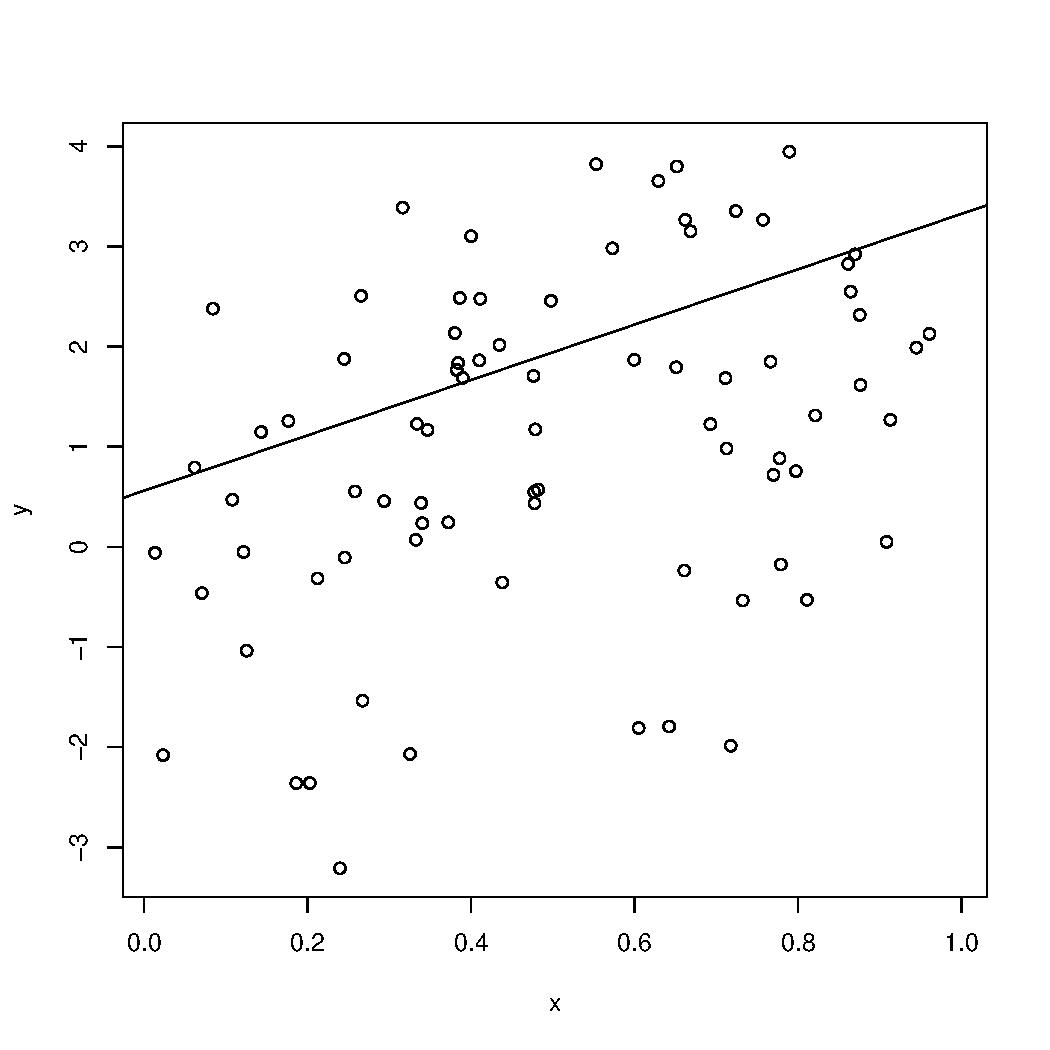
\includegraphics[width=\maxwidth]{figure/unnamed-chunk-5-1} 
\begin{kframe}\begin{alltt}
\hlkwd{rbind}\hlstd{(}\hlkwd{c}\hlstd{(beta0,beta1, sigma2),result1[}\hlnum{1}\hlopt{:}\hlnum{3}\hlstd{])}
\end{alltt}
\begin{verbatim}
##           [,1]     [,2]     [,3]
## [1,] 0.5607442 2.765081 5.313562
## [2,] 0.5180308 2.917809 4.251793
\end{verbatim}
\end{kframe}
\end{knitrout}
\subsection{(d)}
\begin{knitrout}
\definecolor{shadecolor}{rgb}{0.969, 0.969, 0.969}\color{fgcolor}\begin{kframe}
\begin{alltt}
\hlstd{max_logcen} \hlkwb{<-} \hlkwa{function}\hlstd{(}\hlkwc{parb}\hlstd{)\{}
  \hlcom{#put data into the function}
  \hlstd{x} \hlkwb{<-} \hlstd{x}
  \hlstd{y} \hlkwb{<-} \hlstd{y}
  \hlstd{cp} \hlkwb{<-} \hlstd{cp}
  \hlstd{n} \hlkwb{<-} \hlkwd{length}\hlstd{(x)} \hlcom{#length of data}
  \hlstd{cpp} \hlkwb{<-} \hlkwd{which}\hlstd{(}\hlkwd{is.na}\hlstd{(y))} \hlcom{#position of cencoring data}
  \hlstd{ncpp} \hlkwb{<-} \hlkwd{which}\hlstd{(}\hlopt{!}\hlkwd{is.na}\hlstd{(y))} \hlcom{#position of non-cencoring data}
  \hlstd{c} \hlkwb{<-} \hlkwd{length}\hlstd{(cpp)} \hlcom{#length of cencoring data}
  \hlstd{uncen} \hlkwb{<-} \hlkwd{vector}\hlstd{(}\hlstr{"list"}\hlstd{, n}\hlopt{-}\hlstd{c)}
  \hlstd{cen} \hlkwb{<-} \hlkwd{vector}\hlstd{(}\hlstr{"list"}\hlstd{, c)}
  \hlcom{#(need expontial back)}
  \hlstd{s2} \hlkwb{<-} \hlkwd{exp}\hlstd{(parb[}\hlnum{3}\hlstd{])} \hlcom{# since sigma can not be negative, we take log}
  \hlcom{#seperate the log likelihood function into three parts}
  \hlkwa{for}  \hlstd{(i} \hlkwa{in} \hlnum{1}\hlopt{:}\hlstd{n}\hlopt{-}\hlstd{c)\{}
    \hlcom{#non-censoring part}
    \hlstd{uncen[i]} \hlkwb{<-} \hlopt{-}\hlnum{1}\hlopt{/}\hlnum{2}\hlopt{/}\hlstd{s2}\hlopt{*}\hlstd{(y[ncpp[i]]}\hlopt{-}\hlstd{parb[}\hlnum{1}\hlstd{]}\hlopt{-}\hlstd{parb[}\hlnum{2}\hlstd{]}\hlopt{*}\hlstd{x[ncpp[i]])}\hlopt{^}\hlnum{2}

  \hlstd{\}}
  \hlkwa{for} \hlstd{(i} \hlkwa{in} \hlnum{1}\hlopt{:}\hlstd{c)\{}
    \hlcom{#censoring part}
    \hlstd{cen[i]} \hlkwb{<-} \hlkwd{log}\hlstd{(}\hlnum{1}\hlopt{-} \hlkwd{pnorm}\hlstd{((cp}\hlopt{-}\hlstd{parb[}\hlnum{1}\hlstd{]}\hlopt{-}\hlstd{parb[}\hlnum{2}\hlstd{]}\hlopt{*}\hlstd{x[cpp[i]])}\hlopt{/}\hlkwd{sqrt}\hlstd{(s2)))}
  \hlstd{\}}

  \hlstd{logfun} \hlkwb{<-} \hlopt{-}\hlstd{(n}\hlopt{-}\hlstd{c)}\hlopt{/}\hlnum{2}\hlopt{*}\hlkwd{log}\hlstd{(}\hlnum{2}\hlopt{*}\hlstd{pi)}\hlopt{-}\hlstd{(n}\hlopt{-}\hlstd{c)}\hlopt{/}\hlnum{2}\hlopt{*}\hlkwd{log}\hlstd{(s2)}\hlopt{+}\hlkwd{sum}\hlstd{(}\hlkwd{unlist}\hlstd{(uncen))}\hlopt{+}\hlkwd{sum}\hlstd{(}\hlkwd{unlist}\hlstd{(cen))}
  \hlkwd{return}\hlstd{(}\hlopt{-}\hlstd{logfun)}
\hlstd{\}}

\hlstd{start} \hlkwb{<-} \hlkwd{c}\hlstd{(}\hlnum{1}\hlstd{,}\hlnum{1}\hlstd{,}\hlkwd{log}\hlstd{(}\hlnum{3}\hlstd{))} \hlcom{#start point}
\hlcom{#use BFGS method to calculate and try parscale}
\hlstd{(result2} \hlkwb{<-} \hlkwd{optim}\hlstd{(}\hlkwc{par}\hlstd{=start,} \hlkwc{fn}\hlstd{=max_logcen,} \hlkwc{method} \hlstd{=} \hlstr{"BFGS"}\hlstd{,}\hlkwc{control} \hlstd{=} \hlkwd{list}\hlstd{(}\hlkwc{trace} \hlstd{=} \hlnum{TRUE}\hlstd{,} \hlkwc{parscale} \hlstd{=} \hlkwd{c}\hlstd{(}\hlnum{1}\hlstd{,}\hlnum{1}\hlstd{,}\hlnum{100}\hlstd{)))}\hlopt{$}\hlstd{par)}
\end{alltt}
\begin{verbatim}
## initial  value 203.079711 
## final  value 194.276775 
## converged
## [1] 0.4948443 2.7554372 1.5402094
\end{verbatim}
\begin{alltt}
\hlcom{#try nlm and optim to compare the result}
\hlkwd{nlm}\hlstd{(max_logcen,}\hlkwd{c}\hlstd{(}\hlnum{1}\hlstd{,}\hlnum{1}\hlstd{,}\hlnum{3}\hlstd{))}\hlopt{$}\hlstd{estimate}
\end{alltt}
\begin{verbatim}
## [1] 0.4947069 2.7556863 1.5392725
\end{verbatim}
\begin{alltt}
\hlkwd{optim}\hlstd{(}\hlkwd{c}\hlstd{(}\hlnum{1}\hlstd{,}\hlnum{1}\hlstd{,}\hlnum{3}\hlstd{),max_logcen)}\hlopt{$}\hlstd{par}
\end{alltt}
\begin{verbatim}
## [1] 0.4942796 2.7560622 1.5391427
\end{verbatim}
\begin{alltt}
\hlkwd{rbind}\hlstd{(result1[}\hlnum{1}\hlopt{:}\hlnum{3}\hlstd{],}\hlkwd{c}\hlstd{(result2[}\hlnum{1}\hlopt{:}\hlnum{2}\hlstd{],}\hlkwd{exp}\hlstd{(result2[}\hlnum{3}\hlstd{])))}
\end{alltt}
\begin{verbatim}
##           [,1]     [,2]     [,3]
## [1,] 0.5180308 2.917809 4.251793
## [2,] 0.4948443 2.755437 4.665567
\end{verbatim}
\begin{alltt}
\hlcom{#As showing above, the result is quite similar, we can conclude that both methods work.}
\end{alltt}
\end{kframe}
\end{knitrout}

\end{document}
